\section{Versuchsaufbau}
\label{sec:Versuchaufbau}
Der Aufbau des in Kapitel \ref{sec:detektor} beschriebenen Germaniumdetektors ist in Abbildung \ref{fig:aufbauDetektor} dargestellt.
\begin{figure}
  \centering
  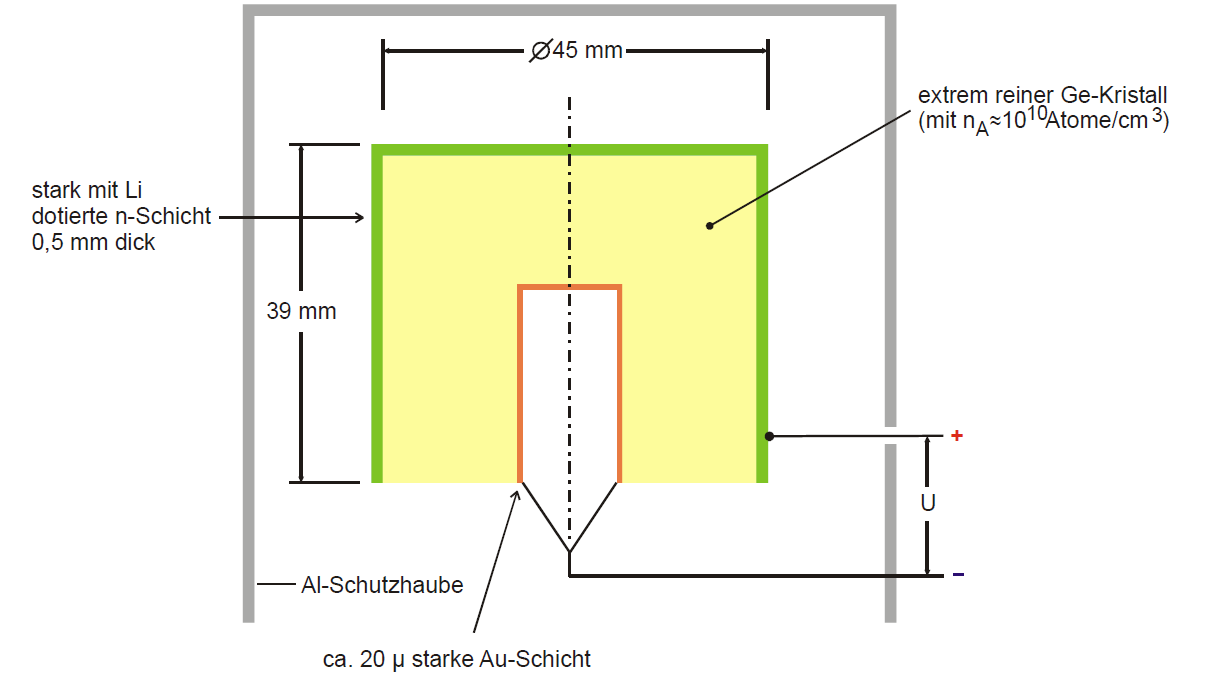
\includegraphics[width=0.8\textwidth]{ressources/aufbauDetektor.png}
  \caption{Querschnitt des Germaniumdetektors, \cite{skript}.}
  \label{fig:aufbauDetektor}
\end{figure}
Außen befindet sich eine Al-Schutzhaube. Aluminium wird hier deshalb gewählt, weil es aufgrund seiner geringen Kernladungszahl vergleichsweise wenig zur Abschirmung des Detektors vor der Strahlungsquelle beiträgt. Die Quelle befindet sich in einem Abstand $a$ oberhalb des Detektors. Somit ergibt sich für den in Kapitel \ref{sec:effizienz} eingeführten Raumwinkel
\begin{equation}
  \Omega = 2\pi \left( 1 - \frac{a}{\sqrt{a^2+r^2}} \right) \; .
  \label{eq:raumwinkel}
\end{equation}
Hierin ist $r$ der Radius des Detektors, also gemäß Abbildung \ref{fig:aufbauDetektor} $r=\SI{22.5}{\milli\meter}$. Es ist zu beachten, dass der Abstand $a$ sich aus dem Abstand zwischen Quelle und Aluminium-Schutzhaube und dem Abstand zwischen Aluminium-Schutzhaube und Verarmungszone zusammensetzt. Letzterer wird mit $\SI{1.5}{\centi\meter}$ abgeschätzt \cite{skript}.\\
Die Kühlung des Detektors erfolgt mit Hilfe eines mit flüssigem Stickstoff gefülltem Dewar-Gefäßes, sodass der Detektor bei ca. $\SI{77}{\kelvin}$ betrieben wird. Ferner wird gleichzeitig der Vorverstärker gekühlt, welcher weiter unten beschrieben wird. Der pn-Übergang besteht aus einer äußeren, stark n-dotierten Schicht von $\SI{0.5}{\milli\meter}$ Dicke. Es grenzt hieran die eigentliche Verarmungszone an in Form des Reinst-Germaniums mit einer geringen p-Dotierung von $n_A\approx10^{10}\si{\per\cubic\centi\meter}$. Die Sperrspannung in Höhe von $\SI{}{\kilo\volt}$ wird zwischen der äußeren n-dotierten Schicht sowie der im inneren liegenden Goldschicht angelegt.\\
Die entstehenden Ladungsimpulse werden mit Hilfe eines Vorverstärkers aufbereitet. Seine Aufgabe ist es, ein der Ladungsmenge proportionales Spannungssignal zu erzeugen. Dazu kommt ein kapazitiv rückgekoppelter Operationsverstärker zum Einsatz, siehe Abbildung \ref{fig:vv}.
\begin{figure}
  \centering
  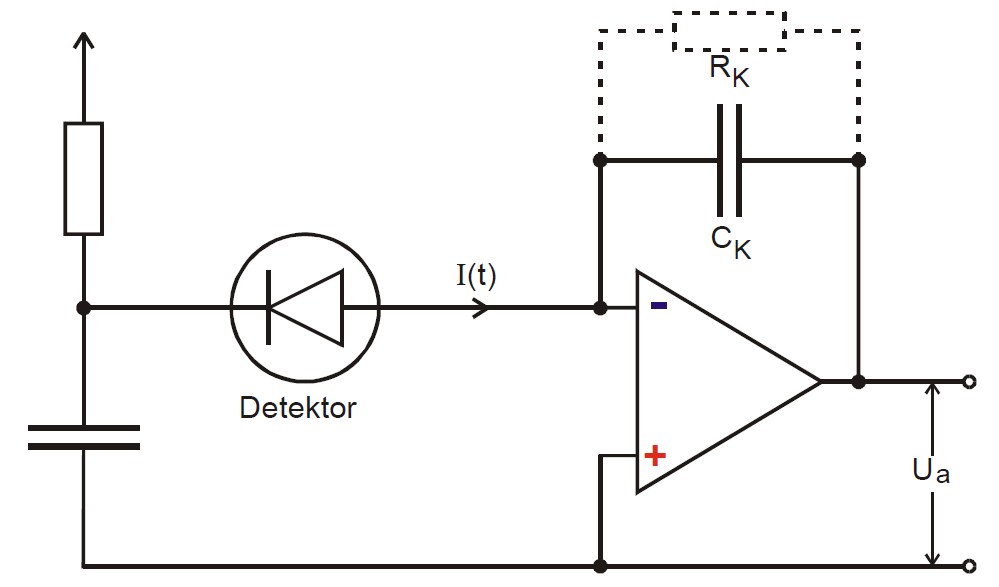
\includegraphics[width=0.7\textwidth]{ressources/vorverstaerker.png}
  \caption{Der Vorverstärker, angeschlossen an den Detektor, \cite{skript}. Der Widerstand $R_K$ wird nicht verwendet, sondern es kommt eine intelligentere Lösung zum Einsatz, um die im Kondensator $C_K$ gesammelte Ladung abfließen zu lassen, siehe Text.}
  \label{fig:vv}
\end{figure}
Die Spannung am Ausgang ergibt sich zu
\begin{equation}
  U_A = -\frac{1}{C_K}\int_0^{t_s}I(t)\text{d}t  \; .
  \label{eq:vvspannung}
\end{equation}
Der Kondensator muss nach jedem Nachweis entladen werden. Dies geschieht hier mit Hilfe einer angesteuerten LED, die die Gate-Drain-Schicht des Feldeffekttransistors im Operationsverstärker kurzzeitig bestrahlt. In diesem Moment wird die Sperrschicht leitend und die Ladung kann abfließen. Diese aufwändig erscheinende Konstruktion wird gewählt, um elektrisches Rauschen zu minimieren. Weitere solcher "Tricks" sind insbesondere im Hauptverstärker verbaut, wiederum mit dem Ziel der Minimierung von Rauschen. Der Hauptverstärker wird an den Vorverstärker angeschlossen (aber außerhalb der Kühlung) und bringt das Spannungssignal auf eine Höhe von ca. $\SI{10}{\volt}$. Das Signal wird schließlich von einem Analog-Digital-Konverter digitalisiert. Die Höhe eines Spannungspulses wird in eine Anzahl von Einzelimpulsen übersetzt. Dabei darf während der Dauer der Konversion kein weiterer Impuls registriert werden, weshalb der Eingang des Konverters solange gesperrt wird. Diese Zeit steht also für die Detektion von Photonen nicht zur Verfügung und wird deshalb als Totzeit bezeichnet. Ihr Wert beläuft sich auf ca. $\SI{40}{\micro\second}$ für große Impulse und entsprechend weniger für kleinere Impulse. Die Anzahl der vom Konverter herausgegebenen Impulse wird mit Hilfe eines Adressregisters in eine von 8192 Kanalnummern übersetzt und in einem Speicher  der entsprechende Counter für diesen Kanal um eins erhöht. Schließlich werden die Daten an einen Computer übertragen und mit Hilfe einer Software direkt das Spektrum dargestellt. Dabei wird jeder Kanalnummer ihr entsprechender Counter zugeordnet.
